% !TEX root = task-2-6-4.tex
% Editable task bank. Append new BankTask blocks at the end of the document.
\documentclass[12pt,a4paper]{article}
\usepackage{physics-textbook}
\usepackage{graphicx,needspace}
\usetikzlibrary{decorations.pathmorphing}
\newif\ifShowSolutions
\ifdefined\TutorEdition
  \ShowSolutionstrue
\else
  \ShowSolutionsfalse % Change to \ShowSolutionstrue to display solutions.
\fi
\newcounter{banktask}
\newsavebox{\BankTaskBox}
\newcommand{\BankTaskContent}[3]{%
  \noindent\textbf{\thebanktask.}\quad #2\par
  \ifShowSolutions
    \Needspace{50mm}% Keep the solution heading with its opening text or diagram.
    #3\par
    \ifdefined\TutorEdition
      \ifcsname TutorSource#1\endcsname
        \nopagebreak\smallskip{\small\csname TutorSource#1\endcsname\par}%
      \fi
    \fi
  \fi
}
\newcommand{\BankTask}[3]{%
  \refstepcounter{banktask}\par\medskip
  \sbox{\BankTaskBox}{\begin{minipage}{\linewidth}%
    \BankTaskContent{#1}{#2}{#3}\end{minipage}}%
  \ifdim\dimexpr\ht\BankTaskBox+\dp\BankTaskBox\relax>\dimexpr\textheight-20mm\relax
    \Needspace{35mm}\BankTaskContent{#1}{#2}{#3}%
  \else
    \Needspace{\dimexpr\ht\BankTaskBox+\dp\BankTaskBox\relax}%
    \noindent\usebox{\BankTaskBox}\par
  \fi
  \medskip
}
\begin{document}
\BookSubsection{2.6.4}{Изобарный процесс}


% Source sdamgia-43309: https://phys-ege.sdamgia.ru/problem?id=43309
\BankTask{sdamgia-43309}{
Температура идеального газа при постоянном давлении увеличилась в $2$ раза. При этом объем увеличился на $150$ $\text{дм}^{3}$. Чему равен начальный объем, занимаемый идеальным газом? (В кубических дециметрах.)
}{
\smallskip\noindent\textbf{Решение}\par
При изобарном процессе $\frac{V_1}{T_1} = \frac{V_2}{T_2} ,$ откуда следует, что при увеличении температуры в $2$ раза его объем увеличился в $2$ раза. Тогда получаем равенство $2V_1=V_1 + \Delta V,$ откуда первоначальный объем $V_1=\Delta V=150\text{дм} ^{3} .$

Ответ: $150$.
}

% Source sdamgia-43814: https://phys-ege.sdamgia.ru/problem?id=43814
\BankTask{sdamgia-43814}{
В вертикальном цилиндре под поршнем находится $2\,\text{моль}$ гелия. Поршень может перемещаться в цилиндре без трения. Масса гелия в цилиндре постоянна. Атмосферное давление считать постоянным.  

$1$) При сжатии гелия в цилиндре внешние силы совершают отрицательную работу.

$2$) При медленном повышении температуры давление гелия в сосуде увеличивается.

$3$) При медленном понижении температуры сила давления гелия на поршень не изменяется.

$4$) Если на поршень насыпать некоторое количество песка, не меняя температуры гелия, то давление гелия после того, как система придёт в равновесие, будет равно первоначальному давлению.

$5$) При медленном повышении температуры объём, занимаемый гелием, увеличивается.
}{
\smallskip\noindent\textbf{Решение}\par
$1$) Неверно. При сжатии гелия в цилиндре объем газа уменьшается, поэтому внешние силы совершают положительную работу.

$2$) Неверно. Так как поршень может перемещаться без трения, то он будет двигаться до тех пор, пока сила давления гелия не станет равной сумме силы тяжести поршня и силы атмосферного давления. Следовательно, при медленном нагревании давление гелия не изменится.

$3$) Верно. При медленном нагревании гелия давление газа не изменится.

$4$) Неверно. Так как сила давления гелия равна сумме силы тяжести поршня и силы атмосферного давления, то при насыпании песка на поршень сила тяжести увеличится, что приведет к увеличению давления гелия.

$5$) Верно. При медленном повышении температуры гелия при изобарном процессе объем увеличится.

Ответ: $35$.
}

% Source sdamgia-2608: https://phys-ege.sdamgia.ru/problem?id=2608
\BankTask{sdamgia-2608}{
В сосуде под поршнем находится идеальный газ. Если при нагревании газа его давление остается постоянным, то как изменятся величины: объем газа, его плотность и внутренняя энергия?

$1$. Увеличилась.

$2$. Уменьшилась.

$3$. Не изменилась.

\begin{center}\begin{tabular}{|p{0.287\linewidth}|p{0.287\linewidth}|p{0.287\linewidth}|}\hline
Объем газа & Плотность газа & Внутренняя энергия газа\\\hline
\strut & \strut & \strut\\\hline\end{tabular}\end{center}
}{
\smallskip\noindent\textbf{Решение}\par
Идеальный газ в сосуде нагревается изобарически. Следовательно, согласно закону Гей-Люссака $( \frac{V}{T} =const ) ,$ объем газа увеличивается. Плотность обратно пропорциональна объему, и, так как количество газа не меняется, плотность газа уменьшается. Внутренняя энергия фиксированного количества идеального газа зависит только от температуры. При повышении температуры внутренняя энергия идеального газа увеличивается $( \Delta U= \frac{i}{2} \nu R\Delta T ) .$

Ответ: $121$.
}

% Source sdamgia-6065: https://phys-ege.sdamgia.ru/problem?id=6065
\BankTask{sdamgia-6065}{
Идеальный газ в количестве $\nu$ молей, имеющий концентрацию $n$ и находящийся при давлении $p$, сначала изобарически сжимают в $2$ раза, а затем изотермически расширяют в $4$ раза. Чему будут равны объем и температура этого газа в конце процесса расширения?

($k$ — постоянная Больцмана, $N_{A}$ — число Авогадро)

\TaskMatchingColumns{Величины}{А)  объем газа в конце процесса расширения\par Б)  температура газа в конце процесса\par расширения}{Их значения}{$1 ) \frac{\nu N_{\text{А}}}{2n}$\par $2 ) \frac{p}{2nk}$\par $3 ) \frac{2 \nu N_{\text{А}}}{n}$\par $4 ) \frac{2p}{nk}$}

\begin{center}\begin{tabular}{|c|c|}\hline
А & Б\\\hline
\strut & \strut\\\hline\end{tabular}\end{center}
}{
\smallskip\noindent\textbf{Решение}\par
Рассмотрим последовательно оба процесса.

$1$-$2$: изобарическое сжатие $p=const.$ В изобарическом процессе отношение $\frac{V}{T}$ остается постоянным. Следовательно, $T_2= \frac{V_2}{V_1} T_1= \frac{1}{2} T_1.$

$2$-$3$: изотермическое расширение $T=const.$ То есть $T_3=T_2= \frac{1}{2} T_1.$ В изотермическом процессе произведение $pV$ остается постоянным. Следовательно, $p_3=p_2 \frac{V_2}{V_3} = \frac{1}{4} p_1.$

Рассмотрим изменение объема в результате двух приведенных процессов: 

$V_2= \frac{1}{2} V_1,V_3=4V_2=2V_1.$

Концентрация $n= \frac{N}{V} ,$ следовательно, $n_3= \frac{1}{2} n_1.$ Теперь выразим искомые величины через величины, данные в условии задачи. Температура и давление идеального газа связаны соотношением $p=nkT.$ Откуда:

$T_3= \frac{p_3}{n_3k} = \frac{\frac{1}{4} p_1}{\frac{1}{2} n_1k} = \frac{p}{2nk}$ (Б — $2$).

Объем газа в конце процесса расширения найдем из уравнения Менделеева — Клапейрона:

$p_1V_1=\nu RT_1 \Longleftrightarrow V_1= \frac{\nu RT_1}{p_1} ,$

$V_3=2V_1= \frac{2\nu RT_1}{p_1} = \frac{2\nu R \frac{p_1}{n_1k}}{p_1} = \frac{2\nu N_{\text{А}}}{n}$ (А — $3$).

Ответ: $32$.
}

% Source sdamgia-12858: https://phys-ege.sdamgia.ru/problem?id=12858
\BankTask{sdamgia-12858}{
В сосуде объемом $250\,\text{л}$ под тяжелым поршнем находится кислород. Давление кислорода $300\,\text{кПа}$. В изобарном процессе плотность газа уменьшилась в $5$ раз. Какую работу совершил газ в этом процессе? (В килоджоулях.)
}{
\smallskip\noindent\textbf{Решение}\par
Поскольку плотность газа уменьшилась в $5$ раз, его объем увеличился в $5$ раз и стал $5\cdot 250=1250\,\text{л}$. Работа газа в изобарном процессе равна

$A=p\Delta V=300 \cdot 10 ^{3} \cdot ( 1250 - 250 ) \cdot 10 ^{- 3} =300 \cdot 10 ^{3} \text{Дж}=300\text{кДж}.$

Ответ: $300$.
}

% Source sdamgia-11267: https://phys-ege.sdamgia.ru/problem?id=11267
\BankTask{sdamgia-11267}{
В изобарном процессе теплоемкость одного моля кислорода равна $29{,}085\,\text{Дж}/\text{К}$. Определите удельную теплоемкость кислорода в этом процессе. (В джоулях на килограмм на Кельвин; округлите до целого числа.)
}{
\smallskip\noindent\textbf{Решение}\par
Удельная теплоемкость вещества по определению есть:

$c= \frac{C}{m} ,$

где $m=\nu M$ — масса вещества, которая выражается через число молей и молярную массу.

Определим удельную теплоемкость кислорода:

$c= \frac{C}{\nu M} = \frac{29{,}085}{1 \cdot 0{,}032} \approx 909 \frac{\text{Дж}}{\text{кг} \cdot \text{К}} .$

Ответ: $909$.
}

% Source sdamgia-12962: https://phys-ege.sdamgia.ru/problem?id=12962
\BankTask{sdamgia-12962}{
Внутренняя энергия одного моля газообразного метана в $2{,}5$ раза больше внутренней энергии такого же количества идеального одноатомного газа при той же температуре. Какое количество теплоты необходимо затратить для того, чтобы изобарически нагреть $0{,}1$ моля газообразного метана на $100\,\text{К}$? (В джоулях; округлите до целого числа.)
}{
\smallskip\noindent\textbf{Решение}\par
В изобарическом процессе $A=p\Delta V=\nu R\Delta T$ и с учетом условия, что внутренняя энергия метана в $2{,}5$ раза больше внутренней энергии такого же количества вещества идеального одноатомного газа при той же температуре, по первому закону термодинамики

$Q=\Delta U + A=2{,}5 \cdot \frac{3}{2} \nu R\Delta T + \nu R\Delta T= ( 3{,}75 + 1 ) \nu R\Delta T=4{,}75 \cdot 0{,}1 \cdot 8{,}31 \cdot 100 \approx 395\text{Дж}.$

Ответ: $395$.
}

% Source sdamgia-3442: https://phys-ege.sdamgia.ru/problem?id=3442
\BankTask{sdamgia-3442}{
Идеальный газ изобарно нагревают так, что его температура изменяется на $\Delta T=240\text{К},$ а объем — в $1{,}4$ раза. Масса газа постоянна. Какова начальная температура газа по шкале Кельвина?
}{
\smallskip\noindent\textbf{Решение}\par
Изобарный процесс — это процесс, проводимый при постоянном давлении. Идеальный газ подчиняется уравнению Клапейрона — Менделеева. В начальном состоянии (до нагревания): $pV_1=\nu RT_1.$ После нагревания: $pV_2=\nu RT_2.$ Вычтя из второго уравнения первое и приняв во внимание, что $V_2=1{,}4V_1,$ получаем соотношение: $p\Delta V=\nu R\Delta T,$ следовательно, $\frac{pV_1}{\nu R} = \frac{\Delta T}{0{,}4} ,$ откуда $0{,}4pV_1=\nu R\Delta T.$

Тогда начальная температура газа равна $T_1= \frac{pV_1}{\nu R} = \frac{\Delta T}{0{,}4} = \frac{240\text{К}}{0{,}4} =600\text{К}.$

Ответ: $600\,\text{К}$.
}

% Source sdamgia-11893: https://phys-ege.sdamgia.ru/problem?id=11893
\BankTask{sdamgia-11893}{
Постоянную массу идеального одноатомного газа изобарно сжали так, что $T_2 = \frac{T_1}{k} .$ Затем этот же газ адиабатически расширяется так, что $T_3 = \frac{T_2}{2} .$ Отношение модулей работ в изобарном и адиабатическом процессах $n = 4.$ Найдите $k$.
}{
\smallskip\noindent\textbf{Решение}\par
Работа, совершенная над газом при изобарном сжатии, вычисляется по формуле: $A_1 = p|\Delta V|.$ Из уравнения Менделеева — Клапейрона для первого и второго состояния газа $p_1V_1 = \nu RT_1$ и $p_2V_2 = \nu RT_2$ получаем:

$A_1 = p ( V_1 - V_2 ) = \nu R ( T_1 - T_2 ) = \nu R ( T_1 - \frac{T_1}{k} ) = \frac{k - 1}{k} \nu RT_1.$

Согласно первому началу термодинамики при адиабатическом расширении работа газа равна $A_2 = - \Delta U,$ откуда:

$A_2 = - \frac{3}{2} \nu R ( T_3 - T_2 ) = \frac{3}{2} \nu R ( T_2 - T_3 ) = \frac{3}{4} \nu R T_2 = \frac{3}{4k} \nu RT_1.$

Отношение работ равно $4$:

$\frac{A_1}{A_2} = 4,$ откуда $\frac{k - 1}{k} \cdot \frac{4k}{3} =4,$ следовательно, $k=4$.

Ответ: $4$.
}

% Source sdamgia-6060: https://phys-ege.sdamgia.ru/problem?id=6060
\BankTask{sdamgia-6060}{
В теплоизолированном сосуде под поршнем находится $1\,\text{моль}$ гелия при температуре $300\,\text{К}$ (обозначим это состояние системы номером $1$). В сосуд через специальный патрубок с краном добавили еще $2$ моля гелия при температуре $450\,\text{К}$ и дождались установления теплового равновесия. После этого, убрав теплоизоляцию, весь оказавшийся под поршнем газ медленно изобарически сжали, изменив его объем в $2$ раза (обозначим это состояние системы номером $2$). Как и во сколько раз изменилась внутренняя энергия системы при переходе из состояния $1$ в состояние $2$?
}{
\smallskip\noindent\textbf{Решение}\par
Внутренняя энергия $\nu$ молей гелия рассчитывается по формуле $U= \frac{3}{2} \nu R T.$ Пусть энергия добавляемой порции газа $U_1',$ внутренняя энергия двух порций газа, находящихся в сосуде в промежуточном состоянии равна $U'.$ Энергия $U'$ равна сумме внутренних энергий двух порций газа в сосуде:

$U'=U_1 + U_1'$

$\frac{3}{2} ( \nu_1 + \nu_1' ) RT'= \frac{3}{2} R\nu_1 T_1 + \frac{3}{2} R\nu'_1 T_1'$

$T'= \frac{\nu_1T_1 + \nu_1'T_1'}{\nu_1 + \nu_1'}$

В изобарическом процессе отношение объема к температуре остается постоянным$\frac{V'}{T'} = \frac{V_2}{T_2} .$ Откуда:

$\text{Т}_2= \frac{V_2}{V'} T'= \frac{1}{2} \frac{\nu_1T_1 + \nu_1'T_1'}{\nu_1 + \nu_1'} = \frac{1}{2} \frac{1 \cdot 300 + 2 \cdot 450}{1 + 2} =200\text{К}.$

Заметим, что количество вещества во втором состоянии $\nu_2=\nu_1 + \nu_1'.$ Найдем отношение $\frac{U_2}{U_1} :$

$\frac{U_2}{U_1} = \frac{\frac{3}{2} \nu_2RT_2}{\frac{3}{2} \nu_1RT_1} = \frac{\nu_2T_2}{\nu_1T_1} = \frac{3 \cdot 200}{1 \cdot 300} =2.$

При переходе системы из состояния $1$ в состояние $2$ ее энергия увеличилась в $2$ раза.

Ответ $2$.
}


% Source 3845F2: https://ege.fipi.ru/bank/questions.php?search=1&proj=BA1F39653304A5B041B656915DC36B38&qid=3845F2
\BankTask{3845F2}{
Разреженный неон в количестве \(5\ \text{моль}\) изобарно расширяется. Во сколько раз увеличится объём газа при повышении его абсолютной температуры в \(3\) раза?
}{
\smallskip\noindent\textbf{Решение от GPT}\par
При постоянных давлении и количестве вещества \(V/T=\mathrm{const}\), поэтому \(V_2/V_1=T_2/T_1=3\).

Ответ: в \(3\) раза.
}

% Source 90F3B1: https://ege.fipi.ru/bank/questions.php?search=1&proj=BA1F39653304A5B041B656915DC36B38&qid=90F3B1
\BankTask{90F3B1}{
При изобарном расширении постоянной массы гелия при нормальном атмосферном давлении его объём увеличился на $0{,}2\,\text{м}^3$. Определите изменение внутренней энергии гелия. (в $\text{кДж}$).
}{
\smallskip\noindent\textbf{Решение от GPT}\par
Для одноатомного идеального газа $U=\frac32pV$. При постоянном давлении $\Delta U=\frac32p\Delta V=\frac32\cdot10^5\cdot0{,}2=3\cdot10^4\,\text{Дж}=30\,\text{кДж}$. Ответ: $30\,\text{кДж}$.
}

% Source 1B1B5D: https://ege.fipi.ru/bank/questions.php?search=1&proj=BA1F39653304A5B041B656915DC36B38&qid=1B1B5D
\BankTask{1B1B5D}{
При изобарном расширении неона его объём увеличился на \(0{,}4\,\text{м}^3\), а внутренняя энергия увеличилась на \(6\,\text{кДж}\). Определите давление неона. (в $\text{кПа}$).
}{
\smallskip\noindent\textbf{Решение от GPT}\par
Для одноатомного идеального газа \(U=\frac32pV\). При постоянном давлении \(\Delta U=\frac32p\Delta V\), откуда
\[
p=\frac{2\Delta U}{3\Delta V}=\frac{2\cdot6\cdot10^3}{3\cdot0{,}4}=10^4\,\text{Па}=10\,\text{кПа}.
\]
Ответ: \(10\,\text{кПа}\).
}

% Source c17D9F: https://ege.fipi.ru/bank/questions.php?search=1&proj=BA1F39653304A5B041B656915DC36B38&qid=c17D9F
\BankTask{c17D9F}{
В вертикальном цилиндре под поршнем находится \(1\,\text{моль}\) гелия. Поршень может перемещаться в сосуде без трения. Атмосферное давление считать постоянным. Масса гелия в сосуде не изменяется.
\begin{enumerate}
\item При медленном понижении температуры объём, занимаемый гелием, не изменяется.
\item При медленном понижении температуры давление гелия не изменяется.
\item Если на поршень насыпать некоторое количество песка, не меняя температуры гелия, то после установления равновесия в системе давление гелия будет меньше первоначального давления.
\item При медленном повышении температуры сила давления гелия на поршень не изменяется.
\item При медленном изотермическом сжатии гелия в цилиндре он отдаёт окружающим телам некоторое положительное количество теплоты.
\end{enumerate}
}{
\smallskip\noindent\textbf{Решение от GPT}\par
В равновесии \(p=p_{\text{атм}}+Mg/S\), где \(M\) — масса поршня с нагрузкой, \(S\) — площадь поршня.
\begin{enumerate}
\item Неверно: при постоянной нагрузке \(p=\mathrm{const}\), поэтому из \(pV=\nu RT\) следует, что при охлаждении объём уменьшается.
\item Верно: давление определяется неизменной нагрузкой и атмосферным давлением.
\item Неверно: добавление песка увеличивает \(M\), поэтому давление возрастает.
\item Верно: сила давления \(F=pS\) постоянна.
\item Верно: при изотермическом сжатии \(\Delta U=0\), работа газа \(A<0\); следовательно, \(Q=\Delta U+A<0\), газ отдаёт теплоту.
\end{enumerate}
Ответ: \(245\).
}

% Source 65ACC9: https://ege.fipi.ru/bank/questions.php?search=1&proj=BA1F39653304A5B041B656915DC36B38&qid=65ACC9
\BankTask{65ACC9}{
Аргон в количестве $\nu\,\text{моль}$ помещают в открытый сверху сосуд под тяжёлый подвижный поршень и начинают охлаждать. Начальное давление газа — $p_0$. Трением между поршнем и стенками сосуда пренебречь.

Установите соответствие между физическими величинами, характеризующими газ, и формулами, выражающими их зависимость от абсолютной температуры $T$ газа ($R$ — универсальная газовая постоянная).

\begin{center}
\TaskMatchingColumns[.53\linewidth]{Физические величины}{
А) объём газа $V(T)$\par
Б) внутренняя энергия газа $U(T)$
}{Формулы}{
1) $\dfrac{\nu RT}{p_0}$\par
2) $\dfrac{\nu Rp_0}{T}$\par
3) $\dfrac{3}{2}\nu RT$\par
4) $\dfrac{3}{2}\dfrac{\nu RT}{p_0}$
}
\end{center}

\begin{center}
\begin{tabular}{|c|c|}\hline
А & Б \\ \hline
\phantom{00} & \phantom{00} \\ \hline
\end{tabular}
\end{center}
}{
\smallskip\noindent\textbf{Решение от GPT}\par
Тяжёлый подвижный поршень поддерживает постоянное давление $p=p_0$. Из уравнения состояния $p_0V=\nu RT$ получаем $V(T)=\dfrac{\nu RT}{p_0}$: А — 1. Аргон — одноатомный идеальный газ, поэтому $U(T)=\dfrac{3}{2}\nu RT$: Б — 3.

Ответ: А — 1, Б — 3.
}

% Source 298FF1: https://ege.fipi.ru/bank/questions.php?search=1&proj=BA1F39653304A5B041B656915DC36B38&qid=298FF1
\BankTask{298FF1}{
\begin{center}
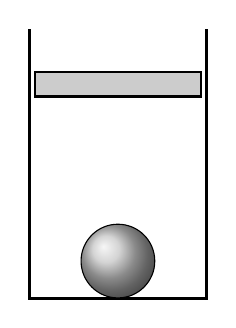
\begin{tikzpicture}[>=stealth,scale=0.9]
\draw[line width=1.2pt] (0,3.8)--(0,0)--(2.5,0)--(2.5,3.8);
\filldraw[fill=gray!40,line width=0.9pt] (0.08,2.85) rectangle (2.42,3.2);
\shade[ball color=gray!45] (1.25,0.53) circle (0.52);
\draw (1.25,0.53) circle (0.52);
\end{tikzpicture}
\end{center}
В цилиндрическом сосуде под поршнем находится газ. Поршень не закреплён и может перемещаться в сосуде без трения. На дне сосуда лежит стальной шарик (см. рисунок). Газ нагревают. Как изменятся в результате этого давление газа и действующая на шарик сила Архимеда? Атмосферное давление неизменно.

Для каждой величины определите соответствующий характер изменения:
\begin{enumerate}
\item увеличится
\item уменьшится
\item не изменится
\end{enumerate}
\TaskChangeTable{Давление газа}{Сила Архимеда}
}{
\smallskip\noindent\textbf{Решение от GPT}\par
Равновесие свободного поршня даёт \(p=p_{\text{атм}}+Mg/S\), где \(M\) — масса поршня, \(S\) — его площадь. Поэтому давление не изменится (\(3\)). При нагревании газ расширяется, его плотность \(\rho\) уменьшается. Следовательно, сила Архимеда \(F_A=\rho gV_{\text{ш}}\) уменьшится (\(2\)).

Ответ: \(32\).
}

% Source 0D4FC9: https://ege.fipi.ru/bank/questions.php?search=1&proj=BA1F39653304A5B041B656915DC36B38&qid=0D4FC9
\BankTask{0D4FC9}{
При исследовании изопроцессов использовался закрытый сосуд переменного объёма, заполненный неоном и соединённый с манометром. Объём сосуда медленно увеличивают, сохраняя давление неона в нём постоянным. Как изменяются при этом внутренняя энергия и плотность неона в сосуде?

Для каждой величины определите соответствующий характер её изменения:
\begin{enumerate}
\item увеличивается
\item уменьшается
\item не изменяется
\end{enumerate}

\TaskChangeTable{Внутренняя энергия неона в сосуде}{Плотность неона в сосуде}
}{
\smallskip\noindent\textbf{Решение от GPT}\par
Для одноатомного идеального газа \(U=\frac32\nu RT=\frac32pV\). При постоянном давлении увеличение объёма приводит к увеличению внутренней энергии (1). Масса газа в закрытом сосуде постоянна, поэтому плотность \(\rho=m/V\) уменьшается (2).

\(\boxed{12}\).
}

% Source c70327: https://ege.fipi.ru/bank/questions.php?search=1&proj=BA1F39653304A5B041B656915DC36B38&qid=c70327
\BankTask{c70327}{
Необходимо на опыте обнаружить зависимость объёма газа, находящегося в сосуде под подвижным поршнем, от температуры газа. Имеются пять различных сосудов с манометрами и термометрами. Сосуды наполнены одним и тем же газом при различных температурах и давлениях (см. таблицу). Какие два сосуда необходимо взять, чтобы провести это исследование?
\begin{center}
\begin{tabular}{|c|c|c|c|}
\hline
\shortstack{№\\сосуда} & \shortstack{Давление\\газа, \(\text{кПа}\)} & \shortstack{Температура газа\\в сосуде, \({}^{\circ}\mathrm{C}\)} & Масса газа, \(\text{г}\) \\
\hline
\(1\) & \(80\) & \(50\) & \(15\) \\
\hline
\(2\) & \(100\) & \(80\) & \(10\) \\
\hline
\(3\) & \(120\) & \(100\) & \(10\) \\
\hline
\(4\) & \(80\) & \(50\) & \(20\) \\
\hline
\(5\) & \(100\) & \(120\) & \(10\) \\
\hline
\end{tabular}
\end{center}
}{
\smallskip\noindent\textbf{Решение от GPT}\par
Для исследования зависимости объёма от температуры нужно сохранить одинаковыми массу газа и давление, изменив температуру. Из уравнения \(pV=(m/M)RT\) при этих условиях следует \(V/T=\mathrm{const}\). Подходят сосуды 2 и 5: в обоих давление \(100\,\text{кПа}\) и масса газа \(10\,\text{г}\), а температуры различаются. Ответ: 2, 5.
}

% Source 9976: https://phys-ege.sdamgia.ru/problem?id=9976
\BankTask{9976}{
Объем $0{,}1$ литра водорода нагревают при постоянном давлении от $300$ до $3000$ К. При высоких температурах молекулы водорода распадаются на отдельные атомы. На графике показана зависимость доли распавшихся молекул от температуры. Чему равен конечный объем газа?
\begin{center}\begin{tikzpicture}[task graph,>=stealth]\draw[gray!65,xstep=.6,ystep=.6](0,0)grid(5.4,3.6);\draw[->](0,0)--(5.4,0)node[below]{\(T,\,\text{К}\)};\draw[->](0,0)--(0,3.7)node[left]{\(\alpha,\,\%\)};\node[below left]at(0,0){\(0\)};\foreach \x/\t in {1.2/1000,2.4/2000,3.6/3000}{\node[below]at(\x,0){\(\t\)};}\foreach \y/\a in {.6/10,1.2/20,1.8/30,2.4/40}{\node[left]at(0,\y){\(\a\)};}\draw[smooth] plot coordinates{(0,0)(.6,.008)(1.2,.052)(1.8,.16)(2.4,.34)(3,.69)(3.6,1.2)(4.2,1.81)(4.8,2.53)(5.4,3.3)};\end{tikzpicture}\end{center}
}{
\smallskip\noindent\textbf{Решение}\par
В первоначальном состоянии весь водород находился в молекулярном состоянии, и согласно уравнению Менделеева  — Клапейрона:

\[pV_1=\nu RT_1.\]

После нагревания согласно графику $\alpha =20\%$ молекул распадется. При распаде из одной молекулы водорода образуется два атома водорода, значит, в сосуде будет $( 1 - \alpha ) \nu$ молекулярного водорода и $2 \alpha \nu$ атомарного водорода. Общее количество вещества стане равным $( 1 - \alpha ) \nu + 2 \alpha \nu = ( 1 + \alpha ) \nu = 1{,}2\nu,$ и согласно уравнению Менделеева  — Клапейрона:

\[pV_2=1{,}2\nu RT_2.\]

Поделив второе уравнение на первое, получаем:

$\frac{V_2}{V_1} =1{,}2 \frac{T_2}{T_1} =1{,}2 \cdot \frac{3000}{300} =12,$

$V_2=12V_1=12 \cdot 0{,}1=1{,}2\,\text{л}.$

Ответ: $V_2=1{,}2\,\text{л}.$
}

\end{document}
